% Arquivo LaTeX de exemplo de dissertação/tese a ser apresentados à CPG do IME-USP
% 
% Versão 3: Sat Feb 13 15:02:20 BRST 2010
%
% Criação: Jesús P. Mena-Chalco
% Revisão: Fabio Kon e Paulo Feofiloff
%  
% Obs: Leia previamente o texto do arquivo README.txt

% Adicionalmente este formato ha sido modificado para su uso en la presentacion
% de trabajos de fin de curso en la carrera de Ingenieria de sistemas y Ciencias de la 
% computacion en la Universidad Nacional de San Agustin
% Revision : Christian E. Portugal Zambrano
% Version 1: Viernes 11 de Noviembre de 2011

\documentclass[12pt,oneside,a4paper]{book}

% ---------------------------------------------------------------------------- %
% Paquetes 
\usepackage[T1]{fontenc}
\usepackage[spanish]{babel}
%\usepackage[latin1]{inputenc}  % uso de la codificación ISO
\usepackage[utf8x]{inputenc}   % uso de la codificación en  UTF-8
\usepackage[pdftex]{graphicx}           % usamos archivos pdf/png como figuras
\usepackage{setspace}                   % espaciamiento flexible
\usepackage{indentfirst}                % identación del primer párrafo
\usepackage{makeidx}                    % índice remissivo
\usepackage[nottoc]{tocbibind}          % incrementamos la bibliografia/indice/contenido en la tabla de contenidos
%\usepackage{courier}                    % usa o Adobe Courier en lugar de Computer Modern Typewriter
\usepackage{type1cm}                    % fontes realmente escaláveis
\usepackage{listings}                   % para formatear codigo fuente Ej: c++ (Ver el paquete listings)
\usepackage{titletoc}
\usepackage{subfigure} 
\usepackage{multicol}
\usepackage{sidecap} 			%para figuras con el caption a un costado
\usepackage{wrapfig}			 %para imágenes envueltas con texto
\usepackage{rotating}
%\usepackage[bf,small,compact]{titlesec} % cabeceras de los títulos más pequeñas y compactas
\usepackage[fixlanguage]{babelbib}
\usepackage[font=small,format=plain,labelfont=bf,up,textfont=it,up]{caption}
\usepackage[usenames,svgnames,dvipsnames]{xcolor}
\usepackage[a4paper,top=3.5cm,bottom=3.5cm,left=2.5cm,right=2.04cm]{geometry} % margenes
%\usepackage[pdftex,plainpages=false,pdfpagelabels,pagebackref,colorlinks=true,citecolor=black,linkcolor=black,urlcolor=black,filecolor=black,bookmarksopen=true]{hyperref} % links en color negro
\usepackage[pdftex,plainpages=false,pdfpagelabels,pagebackref,colorlinks=true,citecolor=DarkGreen,linkcolor=black,urlcolor=DarkRed,filecolor=green]{hyperref} % links coloridos
%\usepackage[all]{hypcap}                % soluciona el problema con hyperref y capitulos
\usepackage{algorithm} %otros estilos son boxed y plain , depende del gusto
\usepackage{algorithmic}
\usepackage{amsmath} % modo de para agregar funciones matemáticas
% ---------------------------------------------------------------------------- %
% Cabeceras similares a el TAOCP de Donald E. Knuth
\usepackage{fancyhdr}
%Para títulos de capítulos personalizados
%\usepackage[Sonny]{fncychap}
%\usepackage[Lenny]{fncychap}
%\usepackage[Glenn]{fncychap}
%\usepackage[Conny]{fncychap}
%\usepackage[Rejne]{fncychap}
%\usepackage[Bjarne]{fncychap}
%\usepackage[Bjornstrup]{fncychap}
%\pagestyle{fancy}
%\fancyhf{}
%\renewcommand{\chaptermark}[1]{\markboth{\MakeUppercase{#1}}{}}
%\renewcommand{\sectionmark}[1]{\markright{\MakeUppercase{#1}}{}}
%\renewcommand{\headrulewidth}{0pt}

\usepackage{pdfpages} %para agregar PDF externos en el documento actual

%Personalización  del paquete hyperref
\hypersetup{
    bookmarksopen=false,         %mostrar bookmarks bar?
    unicode=false,          % aceptar caracteres no latinos en Acrobat’s bookmarks
    pdftoolbar=false,        % mostrar Acrobat’s toolbar?
    pdfmenubar=false,        % mostrar Acrobat’s menu?
    pdffitwindow=false,     % ajustar ancho de ventana de página cuando sea abierta
    pdfstartview={FitH},    % ajustar ancho de página cuando sea abierta
    pdftitle={Título del trabajo de fin de curso},    % título
    pdfauthor={Autor del trabajo},     % autor
    pdfsubject={Tesis para optar el Título de Ingeniero},   % motivo del documento
    pdfcreator={Ej. Kile 2.0.86},   % creator of the document
    pdfproducer={Ej. LaTex}, % producer of the document
    pdfkeywords={Redes Neuronales;} {Conchas de Abanico;} {Lógica Difusa;} {Funciones de Pertenencia;},% lista de las palabras claves (Muy importante!!!)
    pdfnewwindow=true,      % links en una nueva ventana
}

% ----------------TEOREMAS--------------------------------------------------- %
\usepackage{theorem}
%\setlength{\theorempreskipamount}{1mm}
%\setlength{\theorempostskipamount}{1mm}
%Estilos --
%\theoremstyle{plain}
%\theoremstyle{break}
%\theoremstyle{margin}
%\theoremstyle{marginbreak}
%Tipo de letra--
%\rmfamily, \sffamily, \ttfamily, \mdfamily, \bfseries, \upshape, \itshape, \slshape, \scshape, \normalfont
\theorembodyfont{\sffamily}
%\theoremheaderfont{\bfseries \large}
%TEOREMAS
\newtheorem{definicion}{Definición}
\newtheorem{proposicion}{Proposición}
\input spanishAlgorithmic % mi archivo de traducción
%Para el ambiente itemize
\renewcommand{\labelitemi}{$\bullet$}


% ---------------------------------------------------------------------------- %
\graphicspath{{./figuras/}}             % ruta de las figuras (recomendable)
\frenchspacing                          % arruma o espaço: id est (i.e.) e exempli gratia (e.g.) 
\urlstyle{same}                         % URL con el mismo estilo del texto y no mono-spaced
\makeindex                              % para o índice remisivo
\raggedbottom                           % para no permitir espacios extra en el texto
\fontsize{60}{62}\usefont{OT1}{cmr}{m}{n}{\selectfont}
\cleardoublepage
\normalsize


% ---------------------------------------------------------------------------- %
% Cuerpo del documento
\begin{document}
\frontmatter 
% cabecera para las páginas de las secciones anteriores del capítulo
%\fancyhead[RO]{{\footnotesize\rightmark}\hspace{2em}\thepage}
%\setcounter{tocdepth}{2}
%\fancyhead[LE]{\thepage\hspace{2em}\footnotesize{\leftmark}}
%\fancyhead[RE,LO]{}
%\fancyhead[RO]{{\footnotesize\rightmark}\hspace{2em}\thepage}

\onehalfspacing  % espaciamiento

\thispagestyle{empty}
\begin{center}
  
\rule{\textwidth}{8pt} \\
\Large{\textbf{UNIVERSIDAD NACIONAL DE SAN AGUSTÍN}} \\
\large{\textbf{FACULTAD DE INGENIERÍA DE PRODUCCIÓN Y SERVICIOS}} \\
\large{\textbf{ESCUELA PROFESIONAL DE INGENIERÍA DE SISTEMAS}}\\~\\~\\
  
    
\includegraphics[width=0.3\textwidth]{esc_color.pdf} \\
    \vspace*{1.6cm}
     \textbf{\Large{Modelo de Sistema Experto Neuro-difuso para la Codificación de Conchas de Abanico}}\\
     \vspace*{1.2cm}
     \Large{Tesis presentada por el Bachiller:\\}
     \Large{\textbf{Roy Helbert Pepo Pérez Pinto}}
%    
     \vskip 1cm
     \Large{Para optar el Título Profesional de:}\\
     \LARGE{\textbf{INGENIERO DE SISTEMAS}}
    \vskip 1cm
%    % Programa: Nombre del Programa\\
%      Orientador:  Phd. Jesús P. Mena Chalco\\
%     %Coorientador: Prof. Dr. Nome do Coorientador
% 
   \vskip 0.5cm
%     %\normalsize{Durante el desarrollo de este trabajo el autor recibió el apoyo de
%     %...
    
    \vskip 0.3cm
    \normalsize{Arequipa, Marzo del 2012}
\end{center}

% ---------------------------------------------------------------------------- %
% Página de presentación (sólo para la versión final)
\newpage
\thispagestyle{empty}
    \begin{center}
        \vspace*{2.3 cm}
        \textbf{\Large{Modelo de Sistema Experto Neuro-difuso para la Codificación de Conchas de Abanico}}\\
        \vspace*{2 cm}
    \end{center}

    \vskip 2cm

    \begin{flushright}
    % Este exemplar corresponde à redação\\
    % final da dissertação/tese devidamente corrigida\\
    % e defendida por (Nome Completo do Aluno)\\
    % e aprovada pela Comissão Julgadora.
    %
% 	Esta versão definitiva da tese/dissertação\\
% 	contém as correções e alterações sugeridas pela\\
% 	Comissão Julgadora durante a defesa realizada\\
%     por (Nome Completo do Aluno) em 4/5/2010.
          Esta versión definitiva de tesis\\
          contiene las correcciones y alteraciones sugeridas por la \\
          comisión del jurado durante la defensa realizada\\
          por \textit{Roy Helbert Pepo Pérez Pinto}
    \vskip 2cm

    \end{flushright}
    \vskip 4.2cm

    \begin{quote}
    \noindent Comisión del jurado:
    
    \begin{itemize}
		\item Prof. Presidente del jurado  - EPIS - UNSA 
		\item Prof. 2do Miembro del Jurado - EPIS - UNSA  
		\item Prof. 3er Miembro del Jurado - EPIS - UNSA  
    \end{itemize}
      
    \end{quote}
\pagebreak

\pagenumbering{roman}     % comenzamos a enumerar

% ---------------------------------------------------------------------------- %
% Agradecimientos
\chapter*{Agradecimientos}
A Dios por todo lo que me ha dado, a mi padre por su compañía en momentos tan difíciles, a mi madre una luchadora de corazón, a mis hermanas por su apoyo y comprensión. A mis abuelos, que pusieron su granito de arena en este camino, que Dios los tenga en su gloria. Y en general a todos mis seres queridos por su constante apoyo durante toda mi vida, a mis amigos por su confianza en mí, a pesar que a veces hice lo posible para que la pierdan, y a todos los profesores por sus enseñanzas.
  \begin{quotation}
\textbf{Para empezar un gran proyecto, hace falta valentía. Para terminar un gran proyecto, hace falta perseverancia} 
\end{quotation}



% ---------------------------------------------------------------------------- %
% Resumen
\chapter*{Resumen}
Hoy en día la globalización afecta a todos los países sin importar que sean del primer, segundo mundo o tercer mundo. Esto quiere decir que un producto para que pueda ingresar en el mercado a nivel internacional deberá haber vencido las altas barreras de la globalización. En este sentido cualquier producto alimenticio que quiera ingresar al mercado internacional deberá afrontar los estándares de calidad y producción que este exige, es aquí que los países tercermundistas, como el Perú, tienen serías dificultades para cumplirlos más aun cuando se tiene en frente a países que tienen sus procesos automatizados que no les asegura cumplir con estos estándares pero si se los facilita. En el Perú existen un sin número de productos que buscan su inserción en el mercado internacional entre ellos tenemos a la concha de abanico la cual tiene alta demanda en Francia, Canadá y los Estados Unidos. Gracias a ello en Pisco, una de las principales ciudades exportadoras en el Perú de la concha de abanico, surge la necesidad de automatizar los procesos de producción de conchas de abanico para poder insertar su producto en el mercado internacional, en este sentido entre uno de estos procesos tenemos a la codificación de Conchas de Abanico el cual posee algunas singularidades, resaltando entre ellas el alto grado de subjetividad al momento de designar a un molusco con un grado de calidad (Código), en ocasiones se designa con un código de menor precio a moluscos que tienen probabilidades de ser clasificados con un código de mayor precio y viceversa, ocasionando de este modo pérdidas para alguna de las partes. En este trabajo, se presenta un Modelo de Sistema Experto Neurodifuso, como alternativa para la codificación de Conchas de Abanico, que permita obtener el código de clasificación correspondiente - establecido por la FAO (Food and Agriculture Organization of the United Nations) - al molusco, a partir de su peso en gramos. Adicionalmente este modelo da la opción de modificar manualmente las reglas del proceso de codificación, con el fin de realizar una codificación balanceada del producto. \\
\noindent \textbf{Palabras clave:} Lógica Difusa, Sistemas Expertos, Funciones de Pertenencia, Conchas de Abanico.

% ---------------------------------------------------------------------------- %
% Abstract
% \chapter*{Abstract}
% abstract at english
% 
% \noindent \textbf{Keywords:} keyword1, keyword2, keyword3.
  
% ---------------------------------------------------------------------------- %
% Sumário
\tableofcontents    % imprime el resumen

% ---------------------------------------------------------------------------- %
\chapter{Lista de Abreviaturas}
\begin{tabular}{ll}
         FAO     & Organización para la Agricultura y Alimentación\\
         & (\emph{Food and Agriculture Organization of the United Nations})\\
         FAM    & Memoria Asociativa Difusa (\emph{Fuzzy Associative Memory})\\
         IDE 	 & Entorno de Desarrollo Integrado  (\emph{Integrated Development Environment}) \\
\end{tabular}

% ---------------------------------------------------------------------------- %
\chapter{Lista de Símbolos}
\begin{tabular}{ll}
         $pfc$   & Total de píxeles hacia el centro (\emph{Pixel From Center})\\
         $rpc $  & Total de radianes por píxel (\emph{Radian Per Pixel Pitch})\\
         $ro$    & Error por Radian (\emph{Radian offset})\\
\end{tabular}

% ---------------------------------------------------------------------------- %
% Listas de figuras y tablas, estas son creadas automáticamente
\listoffigures            
\listoftables            

% ---------------------------------------------------------------------------- %
% Capítulos del trabajo
\mainmatter

% cabeceras para las páginas de todos los capítulos
%\fancyhead[RE,LO]{\thesection}

%\singlespacing              % espaciamiento simple
\onehalfspacing            % espaciamiento un y medio
%Aqui podemos incluir mas capítulos o secciones en diferentes archivos
%esto para facilitar la lectura del trabajo
\chapter{Introducción}
\label{cap:introduccion}

% ------------------------------------------------------------------------- %%
\section{Definición del Problema}
\label{sec:ideacentral}
En la ciudad de Pisco existen una cantidad significativa de acuicultores, siendo regulados por la Ley General de Pesca del estado peruano, que cultivan moluscos en determinadas áreas aptas para el crecimiento de conchas de abanico. Estos acuicultores luego de cosechar los moluscos de conchas de abanico ofrecen sus productos a las empresas locales que se encargan de su exportación. Para ello, los acuicultores dejan las conchas de abanico agrupadas en manojos de donde posteriormente la empresa local extrae los moluscos de las valvas para poderlos pesar y calcular el pago respectivo a cada acuicultor. Para el calculo de estos pagos las empresas locales clasifican a los moluscos en grados de calidad que dependen del peso grupal de los moluscos. Este proceso de clasificación de conchas de abanico es llamado Codificación que es una tarea realizada por las personas ``Codificadoras'', quienes basadas en su experiencia designan a cada molusco un determinado código de acuerdo al tamaño y a los intereses de la entidad para la que trabajan, sea entidad proveedora (en ocasiones los acuicultores delegan algunas codificadoras para este proceso que defiendan sus intereses) o compradora (empresa local), en el caso que sea de la entidad proveedora, tratarán que el código sea de mayor precio posible, como ejemplo de ello podemos tener según el Cuadro \ref{tab:tabCodigoMolusco} que un molusco que pese 22.7 gr. puede ser catalogado como código 20/30, en el caso que la ``Codificadora'' sea de la entidad compradora, de lo contrario será catalogado 10/20. Actualmente se trata de equilibrar los intereses poniendo ``Codificadoras'' de ambas entidades para poder codificar de una manera equilibrada y/o balanceada. Cabe mencionar que el código de mayor precio es el 10/20 y el de menor precio, el 60/80. Adicionalmente la globalización busca en las empresas exportadoras que sus productos alimenticios cumplan exigentes estándares de clasificación para que puedan ingresar al determinado mercado. En el Perú la producción de Conchas de Abanico constituye un mercado de exportación con una tendencia creciente \cite{cit:SUNAT}, debiendo de cumplir con estándares de clasificación de calidad relacionados a condiciones  físicas (Peso) del molusco. 

\begin{table}[H]
\centering \caption{\label{tab:tabCodigoMolusco} Códigos de exportación de moluscos Conchas de Abanico}
\begin{center}
\scalebox{0.7}{
	\begin{tabular}{|l|cc|cc|} 
	\hline
	\textbf{Código} & \multicolumn{2}{|c|}{\textbf{Unidades/Libra}} & \multicolumn{2}{c|}{\textbf{Peso (gr.)}} \\ 	
	& Min & Max & Min & Max \\  \hline
	10/20 & -- & 20 & 22.7 & Más \\ 
	20/30 & 21 & 30 & 15.1 & 22.6 \\ 
	30/40 & 31 & 40 & 11.4 & 15 \\  
	40/60 & 41 & 60 &  7.6 & 11.3 \\  
	60/80 & 61 & 80 &  5.7 & 7.5 \\  \hline
	\end{tabular}}
	\\ \scriptsize Fuente: FAO
	\end{center}
\end{table}



\subsection{Variable dependiente e independiente}
La variable independiente en esta investigación la cual puede ser controlada por el autor es \textbf{la Función de Pertenencia Dinámica} la cual nos permitirá influir sobre los resultados de clasificación de cada molusco, en este sentido la variable dependiente sería \textbf{el Código de Clasificación de calidad} asignado a cada molusco procesado. 


\subsection{Indicadores de validez}
El método a utilizar para indicar la validez del presente trabajo son los \textbf{Códigos de Clasificación} proporcionados por la FAO, los cuales serán explicados en detalle en la sección \ref{sec:codigos}.

%% ------------------------------------------------------------------------- %%
\section{Objetivos}
\label{sec:objetivo}

\subsection{Objetivo general}
Determinar los códigos de clasificación para moluscos de una manera automatizada utilizando herramientas de bajo costo como balanzas de bajo costo.
\subsection{Objetivos Primarios}
Para lograr un proceso de estimación de distancia robusto de acuerdo a la propuesta, es necesario que se logren 
resolver los siguientes problemas: 
\begin{enumerate}
	\item item 1
	\item item 2
	\item item 3
	\item item 4
\end{enumerate}

\subsection{Objetivos Secundarios}
Descripción de los objetivos secundarios del trabajo de fin de curso.
\subsection{Demostración y validación del modelo}
Se describe los pasos necesarios para validar el proyecto de fin de curso,así como de las técnicas utilizadas
para lograr tal objetivo.


%% ------------------------------------------------------------------------- %%
\section{Contribuciones}
\label{sec:contribuciones}
Las principales contribuciones de este trabajo se listan como sigue:
\begin{itemize}
  \item item 1
  \item item 2\ldots
 \end{itemize}

%% ------------------------------------------------------------------------- %%
\section{Organización del trabajo}
El presente trabajo de tesis está organizado de la siguiente manera: \\
En el Capítulo~\ref{cap:conceptosprevios} se brinda un marco teórico fundamental e introductorio 
sobre visión computacional, tratamiento de colores en imágenes, rango en imágenes, geometría
proyectiva  y fotogrametría además de presentar los trabajos previos recopilados hasta la actualidad, 
luego en el Capítulo~\ref{cap:calibracion} se explica el modelo 
de cámara Pinhole \index{Pinhole}, el cual es fundamental para el proceso de calibración de cámara y se describen los métodos 
estándares actuales para dicho proceso, también se describe los tipos de distorsiones 
que presentan las lentes de los dispositivos de captura de luz, luego en el Capítulo~\ref{cap:deteccion}  se describe \ldots
      % asociado al archivo: 'introduccion.tex'
%% ------------------------------------------------------------------------- %%
\chapter{Estudio de las  Conchas de Abanico}\index{Estudio de las  Conchas de Abanico}
\label{cap:conchasabanico}


\section{Ubicación y Hábitat}\index{Ubicación y Hábitat}

\section{Descripción biológica}\index{Descripción biológica}

\section{Proceso de extracción y producción}\index{Proceso de extracción y producción}

\section{Problemas identificados}\index{Problemas identificados}



\chapter{Conceptos y Trabajos Previos}
\label{cap:conceptosprevios}
En este capítulo se introducen los conceptos teóricos necesarios y también se introducen las técnicas utilizadas 
en el desarrollo de este trabajo. En la sección~\ref{sec:conceptos} se presentan los conceptos teóricos 
básicos, luego en la sección~\ref{sec:trabajosprevios} se describe una recopilación de los trabajos previos
existentes hasta la actualidad relacionados con el presente trabajo.

\section{Conceptos teóricos}
\label{sec:conceptos}

\subsection{Lógica Difusa y funciones de pertenencia} 
\index{Lógica!Difusa}
En 1965 \cite{cit:zadeh} se aplicó la lógica multivaluada a la teoría de conjuntos, estableciendo la posibilidad de que los elementos pudieran tener diferentes grados de pertenencia a un conjunto.
La lógica difusa (fuzzy logic) refleja muy cercanamente la manera en que razonamos los humanos con reglas aproximadas. Esta es una extensión de la lógica clásica diseñada para permitir  razonamiento sobre conceptos imprecisos. La lógica difusa es una lógica multivaluada que permite una gradación continua en el valor de verdad de una proposición, al poder utilizar cualquier valor en el intervalo [0,1].




\subsection{Códigos de Clasificación de Conchas de Abanico} 
\label{sec:codigos}

\subsubsection{Definiciones básicas}
\begin{definicion}
Si {V} es un espacio vectorial. El espacio proyectivo {P(V)} de {V} es el conjunto de sub-espacios vectoriales 
unidimensionales de {V}.
\end{definicion}

\begin{definicion}
Si el espacio vectorial {V} tiene $n+1$ dimensiones, entonces {P(V)} es un espacio proyectivo de dimensión $n$. 
A un espacio proyectivo unidimensional se le conoce como \textbf{linea proyectiva} (linea de proyección), 
y a un espacio bidimensional se lo define como \textbf{plano proyectivo}.
\end{definicion}

\subsubsection{Subespacios lineales}
\begin{definicion}
Un subespacio lineal del espacio proyectivo {P(V)} es el conjunto de vectores subespaciales unidimensionales de 
un vector subespacial $U \subseteq V$
\end{definicion}


\subsection{Desplazamiento de Funciones} 

\subsection{Sistemas Expertos} 


\subsection{Redes Neuronales} 

\section{Trabajos previos}\index{Trabajos Previos}
\label{sec:trabajosprevios}
Hasta ahora en la literatura se han tratado diversos trabajos relacionados con
la estimación de distancias usando dispositivos tales como una cámara web y un
puntero láser. En el siglo pasado se comenzó a estudiar los fenómenos ocurrentes
en las imágenes digitales, en~\cite{Brown1971} el autor logró establecer la importancia de la
estimación de distancias, estableció un modelo de sistema para obtener medidas cercanas 
fotogramétricas para la obtención de medidas de estructuras\ldots
         
\chapter{Sistema Experto para la Codificación de Conchas de Abanico}\index{Sistema Experto para la Codificación de Conchas de Abanico}
\label{cap:sistemaexperto}
La visión comienza con la captura de la luz\ldots

\section{Reglas Difusas}\index{Reglas Difusas}
\section{Desplazamiento de funciones de pertenencia}\index{Desplazamiento de funciones de pertenencia}
\section{Modelo matemático}\index{Modelo matemático}
\section{Implementación de redes FAM dinámicas}\index{Implementación de redes FAM dinámicas}
\section{Diagrama Entidad-Relación}\index{Diagrama Entidad-Relación}
\section{Diagramas UML}\index{Diagramas UML}



%% ------------------------------------------------------------------------- %%
\chapter{Análisis y Pruebas}\index{Análisis y Pruebas}
\label{cap:pruebas}



\section{Pruebas}
En este capítulo se ha descrito\ldots

	
	

%% ------------------------------------------------------------------------- %%
\chapter{Conclusiones y Trabajos Futuros}\index{Conclusiones y Trabajos Futuros}
\label{cap:conclusiones}


\section{Conclusiones}
En este capítulo se ha descrito\ldots

\section{Trabajos Futuros}


% cabeceras para los apéndices
%\renewcommand{\chaptermark}[1]{\markboth{\MakeUppercase{\appendixname\ \thechapter}} {\MakeUppercase{#1}} }
%\fancyhead[RE,LO]{}
% ---------------------------------------------------------------------------- %

\appendix
\chapter{Software implementado para el sistema}
\label{ape:apendiceC}
En este apartado describiré la aplicación de software utilizada 
para la demostración y validación del este trabajo, la aplicación
fue desarrollada en  el IDE ECLIPSE, como framework para el 
procesamiento de imágenes se utilizó OpenCV, como lenguaje de 
programación nativo se usó c++ y para el diseño de la interfaz de
usuario se utilizó QT. Pasamos a definir los componentes: 

\section{Eclipse IDE}

\begin{wrapfigure}{r}{0.4\textwidth}
  %\begin{center}
    
\includegraphics[width=0.4\textwidth]{apendiceC/eclipse}
  %\end{center}
  %\caption{A gull}
\end{wrapfigure}
 
Eclipse es un entorno de desarrollo integrado de código abierto multiplataforma 
para desarrollar lo que el proyecto llama ``Aplicaciones de Cliente Enriquecido", 
opuesto a las aplicaciones ``Cliente-liviano" basadas en navegadores. 
Esta plataforma, típicamente ha sido usada para desarrollar entornos de desarrollo 
integrados (del inglés IDE), como el IDE de Java llamado Java Development Toolkit (JDT) 
y el compilador (ECJ) que se entrega como parte de Eclipse (y que son usados también 
para desarrollar el mismo Eclipse). Sin embargo, también se puede usar para otros 
tipos de aplicaciones cliente, como BitTorrent o Azureus.
Eclipse es también una comunidad de usuarios, extendiendo constantemente las áreas 
de aplicación cubiertas. Un ejemplo es el recientemente creado Eclipse Modeling 
Project, cubriendo casi todas las áreas de Model Driven Engineering.\\
Eclipse fue desarrollado originalmente por IBM como el sucesor de su familia de 
herramientas para VisualAge. Eclipse es ahora desarrollado por la Fundación Eclipse, 
una organización independiente sin ánimo de lucro que fomenta una comunidad de código 
abierto y un conjunto de productos complementarios, capacidades y servicios.
Eclipse fue liberado originalmente bajo la Common Public License, pero después fue 
re-licenciado bajo la Eclipse Public License. La Free Software Foundation ha dicho 
que ambas licencias son licencias de software libre, pero son incompatibles con 
Licencia pública general de GNU (GNU GPL).3 . Para mayor información puede visitar 
el site del proyecto \url{http://www.eclipse.org/}

\section{OpenCV}

\begin{wrapfigure}{l}{0.2\textwidth}
  %\begin{center}
    
\includegraphics[width=0.2\textwidth]{apendiceC/opencv}
  %\end{center}
  %\caption{A gull}
\end{wrapfigure}

OpenCV es una biblioteca libre de visión artificial originalmente desarrollada por Intel. 
Desde que apareció su primera versión alfa en el mes de enero de 1999, se ha utilizado en 
infinidad de aplicaciones. Desde sistemas de seguridad con detección de movimiento, hasta 
aplicativos de control de procesos donde se requiere reconocimiento de objetos. Esto se 
debe a que su publicación se da bajo licencia BSD, que permite que sea usada libremente 
para propósitos comerciales y de investigación con las condiciones en ella expresadas.
Open CV es multiplataforma, existiendo versiones para GNU/Linux, Mac OS X y Windows. 
Contiene más de 500 funciones que abarcan una gran gama de áreas en el proceso de visión, 
como reconocimiento de objetos (reconocimiento facial), calibración de cámaras, visión 
estereo y visión robótica.\\
El proyecto pretende proporcionar un entorno de desarrollo fácil de utilizar y altamente 
eficiente. Esto se ha logrado, realizando su programación en código C y C++ optimizados, 
aprovechando además las capacidades que proveen los procesadores multi núcleo. OpenCV puede 
además utilizar el sistema de primitivas de rendimiento integradas de Intel, un conjunto 
de rutinas de bajo nivel específicas para procesadores Intel.
Para mayor información ver el site \url{http://opencv.willowgarage.com/wiki/}

\section{Qt}

\begin{wrapfigure}{r}{0.3\textwidth}
  %\begin{center}
    
\includegraphics[width=0.3\textwidth]{apendiceC/qt}
  %\end{center}
  %\caption{A gull}
\end{wrapfigure}

Qt es una biblioteca multiplataforma ampliamente usada para desarrollar aplicaciones con 
una interfaz gráfica de usuario así como también para el desarrollo de programas sin 
interfaz gráfica como herramientas para la línea de comandos y consolas para servidores.
Es producido por la división de software Qt de Nokia, que entró en vigor después de la 
adquisición por parte de Nokia de la empresa noruega Trolltech, el productor original 
de Qt, el 17 de junio de 2008.16 Nokia anuncio que va a detener sus desarrollos en Symbian 
para usar la plataforma de Microsoft para sus telefonos inteligentes en Febrero de 2011.
En marzo del mismo año, anunciaron la adquisición de las licencias comerciales de QT por 
Digia PLC, aunque Nokia va a continuar como la fuerza de desarrollo principal atras de 
la librería.\\
Qt es utilizada en KDE, un entorno de escritorio para sistemas como GNU/Linux o FreeBSD, 
entre otros. Qt utiliza el lenguaje de programación C++ de forma nativa, adicionalmente 
puede ser utilizado en varios otros lenguajes de programación a través de bindings. 
También es usada en sistemas informáticos empotrados para automoción, aeronavegación y 
aparatos domésticos como frigoríficos.
Funciona en todas las principales plataformas, y tiene un amplio apoyo. El API de la 
biblioteca cuenta con métodos para acceder a bases de datos mediante SQL, así como uso 
de XML, gestión de hilos, soporte de red, una API multiplataforma unificada para la 
manipulación de archivos y una multitud de otros para el manejo de ficheros, además de 
estructuras de datos tradicionales.
Distribuida bajo los términos de GNU Lesser General Public License (y otras), Qt es 
software libre y de código abierto. Para mayor información visitar el site 
\url{http://qt.nokia.com/products/}

\section{Descripción de la aplicación}
\begin{figure}[h]
 \centering
  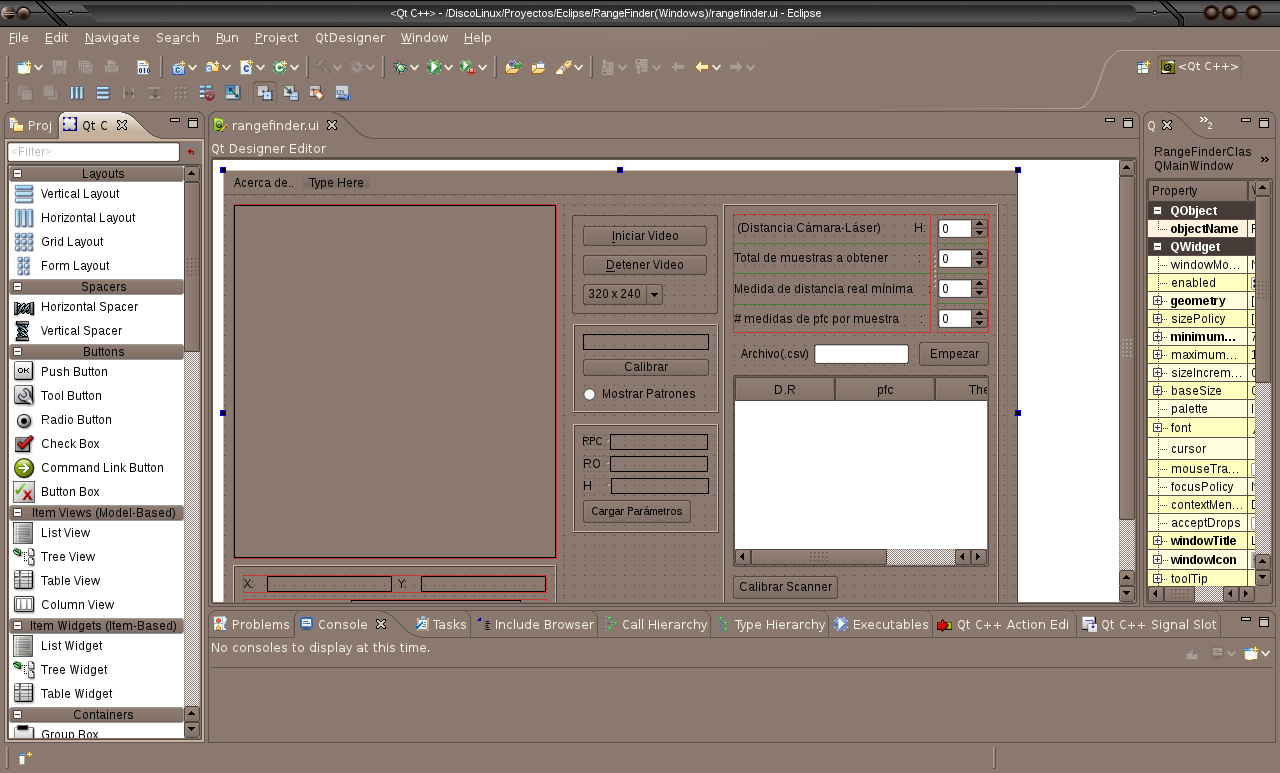
\includegraphics[width=0.7\textwidth]{apendiceC/eclipseintegration}
  \caption{Integración del plugin de Qt para Eclipse, se pueden ver sus cajas de herramientas 
  y su diseñador integrado de interfaces de usuario.}
\label{fig:eclipseintegration}
\end{figure}
El funcionamiento de la aplicación se describe en la Figura \ldots en donde
se puede apreciar el flujo de procesos de la aplicación, el desarrollo de la aplicación se 
hizo en IDE Eclipse Versión Ganymede y la integración de QT con Opencv se llevó a cabo con 
el QT Eclipse Plugin Integration disponible en \url{http://qt.nokia.com/products/eclipse-integration}.
En la Figura \ref{fig:eclipseintegration} podemos ver el plugin de QT integrado en Eclipse, se 
pueden apreciar sus cajas de herramientas y su diseñador integrado de interfaces de usuario.

\subsection{Componentes del sistema}
Para un mejor entendimiento de la estructura de la aplicación se muestra su respectivo Diagrama UML 
de componentes y de clases utilizados en el sistema. 

DIAGRAMA DE COMPONENTES
\begin{figure}[h]
 \centering
  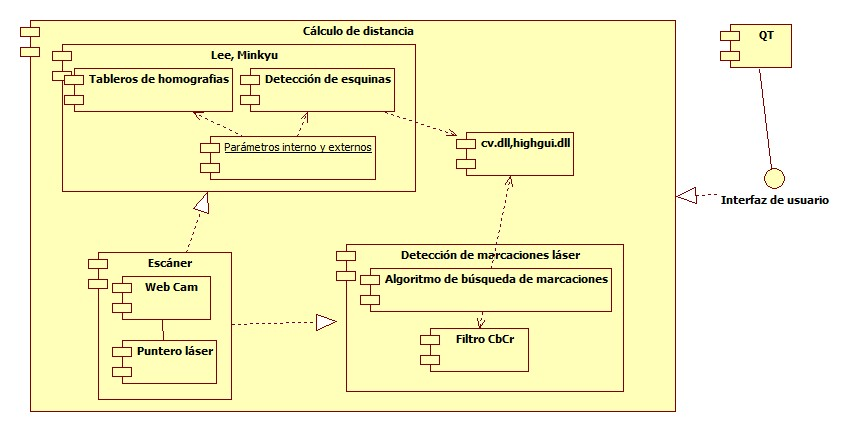
\includegraphics[width=0.9\textwidth]{apendiceC/Componentes}
  \caption{Diagrama de Componentes de la aplicación desarrollado para validación del modelo de estimación de distancia.}
\end{figure}

\begin{sidewaysfigure}
%\begin{figure}[p]
DIAGRAMA DE CLASES
 \centering
  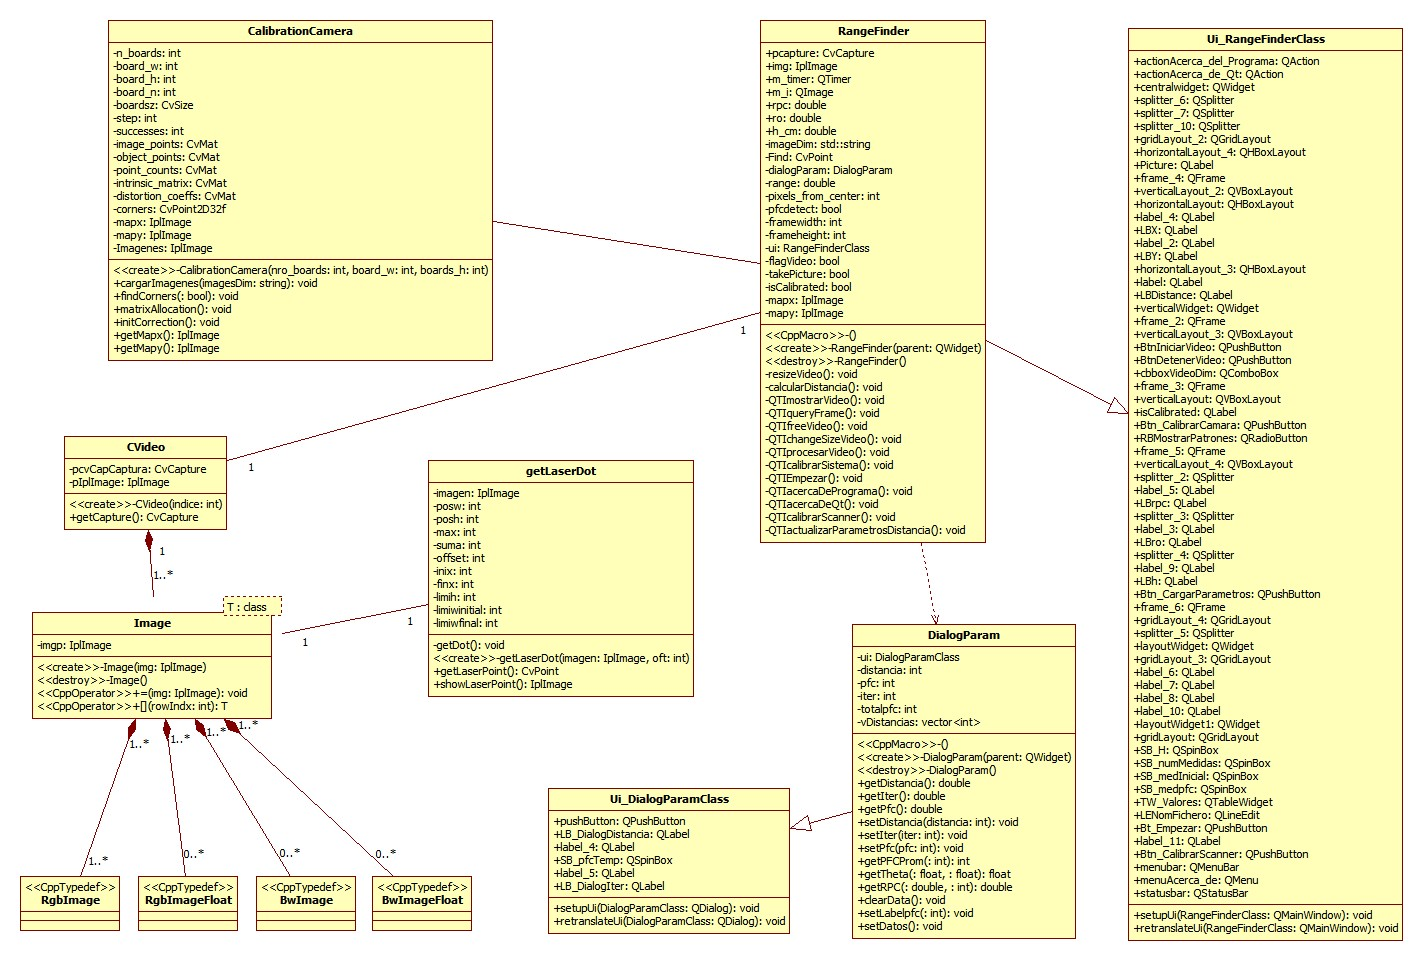
\includegraphics[width=\textwidth]{apendiceC/RangeFinderDiagram}
  \caption{Diagrama de clases de la aplicación desarrollado para validación del modelo de 
estimación de distancia.}
%\end{figure}
\end{sidewaysfigure}





\chapter{Artículo presentado en el Congreso Latinoamericano de Estudiantes en Informática (CLEI). Medellín - Colombia, 2012}
\label{ape:apendiceE}


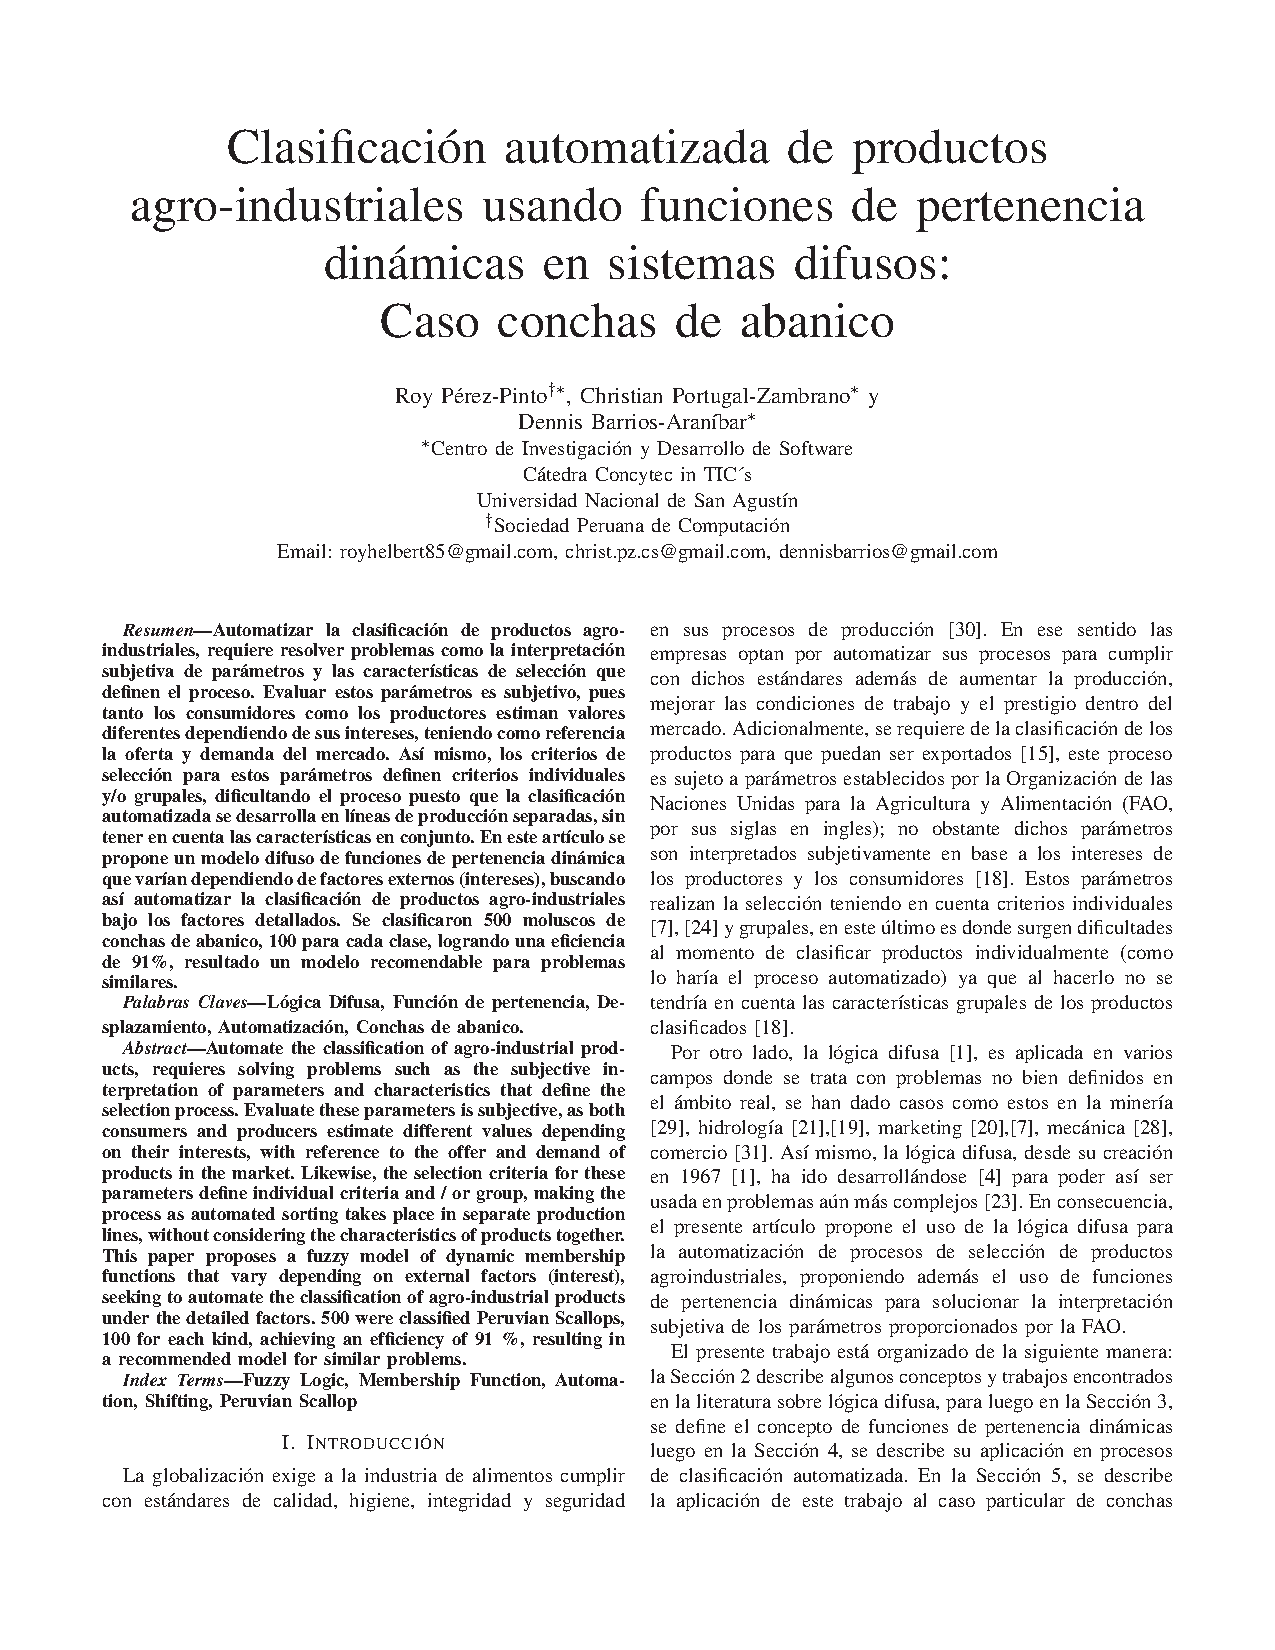
\includepdf[pages=-]{paperCLEI}
%\includepdf[pages=-]{EstDistAbs2011CLEI}
\chapter{Artículo presentado en las Jornadas Peruanas de Computación (JPC). Pucallpa - Perú, 2011}
\label{ape:apendiceD}

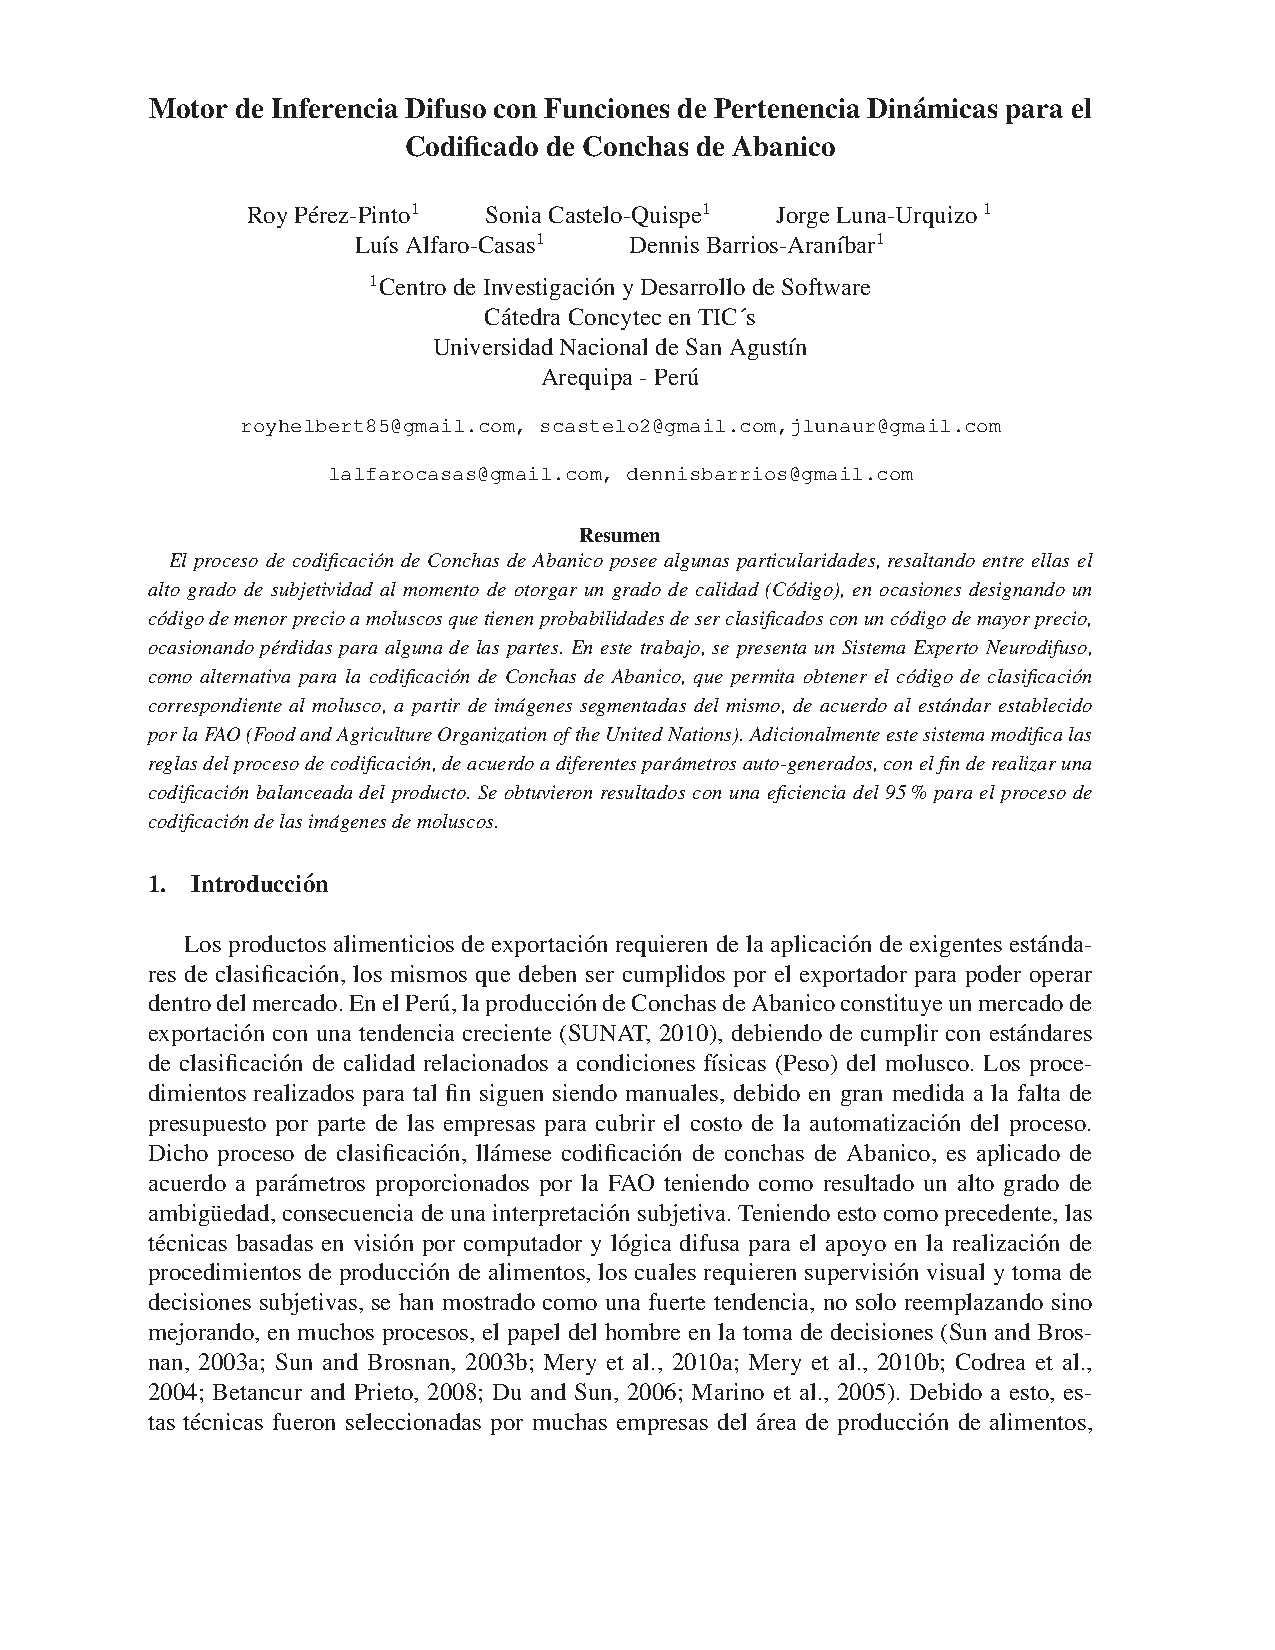
\includepdf[pages=-]{paperJPC}
%\includepdf[pages=-]{EstDistAbs2011CLEI}


% Índice remissivo
\printindex   % imprime el índice alfabético en el documento

% ---------------------------------------------------------------------------- %
% Bibliografia
\backmatter \singlespacing   % espaciamientos simples
\nocite{*}
\bibliographystyle{apalike}% modo de citación bibliográfica
\bibliography{biblioTesisFinal}   %asociado al archivo 'biblioTesisFinal.bib'





\end{document}
